\documentclass[twocolumn,superscriptaddress]{revtex4-1}
\usepackage{graphicx}
\usepackage{epstopdf}
\usepackage{amsmath}
% \usepackage{hyperref}
\usepackage{booktabs}
\usepackage{color}
\usepackage{multirow}
\setlength{\tabcolsep}{10pt}

\begin{document}

\title{Increasing length scales in polydisperse hard spheres: the importance of multi-body correlations.} 

\author{Mathieu Leocmach}
\email{mathieu.leocmach@polytechnique.org}
\altaffiliation[Present address: ]{Laboratoire de Physique, CNRS UMR 5672, Ecole Normale Supérieure de Lyon, 46 allée d'Italie 69364 Lyon cedex 07, France.}
\author{John Russo}
\email{russoj@iis.u-tokyo.ac.jp}
\author{Hajime Tanaka}
\email{tanaka@iis.u-tokyo.ac.jp}
\affiliation{ {Institute of Industrial Science, University of Tokyo, 4-6-1 Komaba, Meguro-ku, Tokyo 153-8505, Japan} }

\date{Received \today}

\begin{abstract}
With numerical simulations of supercooled polydisperse hard spheres systems,
we show that the lengthscale associated with any two-point spatial correlation function
doesn't increase towards the glass transition. An increasing lengthscale is instead revealed
by considering multi-body correlation functions, such as correlators of orientational order.
We also reveal that the stability against crystallization with increasing polydispersity
is due to an increasing population of icosahedral arrangements of particles, competing with bond-orientationally
oriented regions which instead promote crystallization.

\end{abstract}

\maketitle

\section{Introduction}


\section{Methods}
We run isothermal-isobaric NpT Monte Carlo simulations of $N=4000$ polydisperse hard spheres.
The diameters ($\sigma$) follow a Gaussian distribution $P(\sigma)=\exp{\left[-(\sigma-\sigma_0)^2/2\,s^2\right]}/\sqrt{2\pi} s$,
with polydispersity index $\delta=s/\sigma_0$. In the following we fix the unit of length as $\sigma_0=1$.

Our aim is to compare the behaviour of both two-point quantities and multi-body quantities with increasing pressure.
Due to the hard-sphere interaction, entropy is the only contribution to the system free energy.
All two-pair correlation quantities are thus derived from the two-body excess entropy~\cite{Nettleton1958,Mountain1971},
defined as
\begin{equation}
s_2=-\frac{\rho}{2}\int dr\left[g(r)\log(g(r))-g(r)+1\right]
\end{equation}
In principle, $s_2$ can be calculated separately for each particle $i$ in the system. In practice, this requires short time averages to compute the pair correlation function of each particle, $g_i(r)$\cite{tanaka}. We instead construct an approximate but instantaneous $s_2(i)$ using the global $g(r)$
\begin{equation}
s_2(i) = -\frac{\rho}{2}\sum_j \left[g(r_{ij})\log(g(r_{ij}))-g(r_{ij})+1\right].
\end{equation}
This quantity is in very good agreement with the short time average procedure when the averaging time is comparable to the $\beta$ relaxation ; however the results can be very different if the averaging time becomes comparable or longer than the $\alpha$ relaxation, like in Ref.~\cite{tanaka}.

Alternatively, one can compute directly the free-energy of each configuration by
considering the free volume, defined as the volume ($v(i)$) in which each sphere can freely
move while holding all the other spheres fixed. It has been shown~\cite{Aste2004} that this free
volume is simply related to the pair free-energy ($f_2$) by the following relation
\begin{equation}
f_2=\sum_i f_2(i)=-k_BT\sum_i \log(v(i)/\lambda)
\end{equation}
where $\lambda$ is the thermal wavelength. To compute the free volume we follow previous
studies: first the Voronoi-diagram for each configuration is computed, and the Polyhedron
surrounding each particle is determined. The free volume of particle $i$ is then
computed by shifting normally all the faces of the corresponding polyhedron by $\sigma(i)/2$
towards particle $i$, and computing the new volume. This procedure is conducted indipendentely
for each particle and for each configuration.



To study multi-body correlations we use the local bond-order analysis introduced by
\citet{steinhardt}, first applied to study crystal nucleation by
Frenkel and co-workers~\cite{auer}. 
The $\ell$-fold symmetry of a neighbourhood around each particle $i$ is characterised by a $(2\ell+1)$ dimensional complex vector ($\mathbf{q}_l$) as $q_{\ell m}(i)=\frac{1}{N_b(i)}\sum_{j=1}^{N_b(i)} Y_{\ell m}(\mathbf{\hat{r}_{ij}})$, where
$\ell$ is a free integer parameter, and $m$ is an integer
that runs from $m=-\ell$ to $m=\ell$. The functions $Y_{\ell m}$ are the spherical harmonics
and $\mathbf{\hat{r}_{ij}}$ is the vector from particle $i$ to particle $j$.
The sum goes over all neighbouring particles $N_b(i)$ of particle $i$. Usually 
$N_b(i)$ is defined by all particles within a cutoff distance, but in an inhomogeneous system
the cutoff distance would have to change according to the local density. Instead we 
fix $N_b(i)=12$ which is the number of nearest neighbours in icosahedra and close packed crystals (like \textsc{hcp} and \textsc{fcc})
which are known to be the only relevant structures for hard spheres.

In the analysis, one uses the rotational invariants defined as:
\begin{align}
	q_\ell =& \sqrt{\frac{4\pi}{2l+1} \sum_{m=-\ell}^{\ell} |q_{\ell m}|^2 }, \label{eq:ql}\\
	w_\ell =& \sum_{m_1+m_2+m_3=0} 
			\left( \begin{array}{ccc}
				\ell & \ell & \ell \\
				m_1 & m_2 & m_3 
			\end{array} \right)
			q_{\ell m_1} q_{\ell m_2} q_{\ell m_3}. \label{eq:wl}
\end{align}
where the term in brackets in Eq.~(\ref{eq:wl}) is the Wigner 3-j symbol.
In particular both crystalline and icosahedral neighbourhood have high $q_6$ (strong 6-fold symmetry), with the highest values for the later. To detect specifically icosahedral order one prefers $w_6$, whose minimum value is obtained only by a perfect icosahedron. To detect specifically crystal-like order, one should use their extendability: two neighbouring crystal-like neighbourhood should have similar orientation, thus similar vectorial $\mathbf{q}_6$.

The scalar product $(\mathbf{q}_6(i)/|\mathbf{q}_6(i)|)\cdot(\mathbf{q}_6(j)/|\mathbf{q}_6(j)|)$ quantifies this similarity. If it exceeds $0.7$ between
two neighbours, they are deemed \emph{connected}. We then identify a particle as crystalline if it is connected with at least $7$ neighbours~\cite{auer}. In a more continuous way, summing the contribution of all the bonds of a given particle, we define the ``crystallinity''~\cite{russo_hs}
\begin{equation}\label{eqn:crystallinity}
 \text{C}(i)=\sum_{j=0}^{N_b(i)}\frac{\mathbf{q}_6(i)\cdot\mathbf{q}_6(j)}{|\mathbf{q}_6(i)|\,|\mathbf{q}_6(j)|}.
\end{equation}

Alternatively, one can coarse-grain $\mathbf{q}_\ell$ over the neighbours~\cite{lechner}
\begin{equation}
	Q_{\ell m}(i) = \frac{1}{N(i)+1}\left( q_{\ell m}(i) +  \sum_{j=0}^{N(i)} q_{\ell m}(j)\right), 
	\label{eq:Qlm}
\end{equation}
and use the resulting invariant $Q_6$ as an indication of crystallinity.

We note that both $\text{C}$ and $Q_6$ are no direct indicator for the presence of crystals, but rather measures for a tendency to promote crystallisation.

\section{Results}

\begin{figure}
 \centering
 \includegraphics[width=8cm]{./figures/eos.eps}
 % eos.pdf: 682x489 pixel, 72dpi, 24.06x17.25 cm, bb=0 0 682 489
 \caption{Simulated state points. The circles (black curve) represent the equation of state
for polydispersity $\delta=7\%$. The squares (red curve) instead are simulation points at the same
pressure ($\beta p\sigma^3=23$) but at different polydispersities $\delta$: from low to high
volume fraction they correspond to $\delta=7\%,9\%,11\%,13\%,15\%$ respectively.}
 \label{fig:eos}
\end{figure}


Fig.~\ref{fig:eos} shows the equation of state for the simulated state points. In particular
we consider two data-sets. The first one (black circles in the figure) corresponds to
simulations at a constant polydispersity of $\delta=7\%$. For each state point we run $8$ independent
simulation runs and extract configurations for the calculation of correlation lengths.
The second data set (red cicles in the figure) are instead isobaric simulation (at $\beta p\sigma^3=23$)
with increasing polydispersity, $\delta=7\%,9\%,11\%,13\%,15\%$. These state points are used to study
the mechanism by which crystallization is suppressed upon increase of polydispersity, unveiling the
role played by icosahedral arrangement of particles.

\subsection{Order parameter distribution and mobility}

\begin{figure}
	\centering
	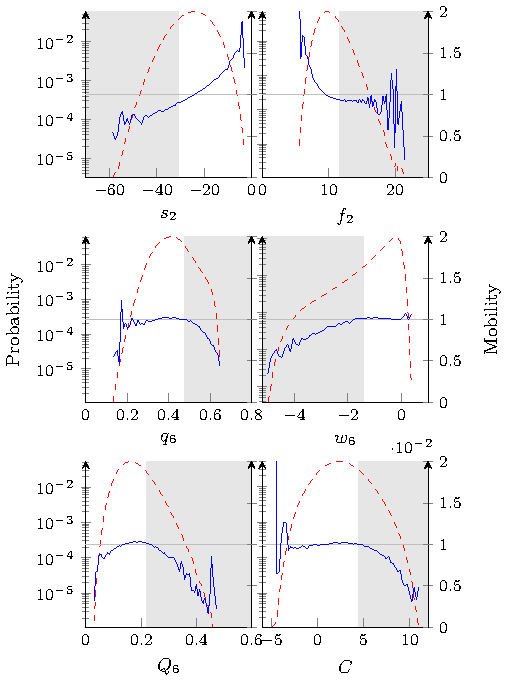
\includegraphics{fig_distrib}
	\caption{\textbf{Probability distribution} (red dash) \textbf{and mobility} (blue continuous) function of various order parameter at $\beta p\sigma^3=25$ and for a time difference corresponding to the $\alpha$-relaxation. Mobility is in unit of mean-square displacement. The limit of the shaded area is at one standard deviation from the mean value of the order parameter in the direction of ordering.}
	\label{fig:distrib}
\end{figure}

We study systematically two-body ($s_2$, $f_2$) and multi-body ($q_6$, $w_6$, $Q_6$, $C$) scalar order parameter fields for our highest pressure ($\beta p\sigma^3=25$). Figure~\ref{fig:distrib} shows the probability distribution of these parameters, always skewed toward the ordered side (shaded in Fig.~\ref{fig:distrib}).

To study the correlation between any scalar order parameter $x$ and the displacement of the particles, we define the mobility 
\begin{equation}
	\Delta r^2(x=x_0, t) \equiv \left\langle \frac{
		\sum\limits_i{
			\left\|\mathbf{r}_i(t)-\mathbf{r}_i(0)\right\|^2 \delta(x(i)-x_0)
			}
	}{
		\sum\limits_i{\delta(x(i)-x_0)}
	}\right\rangle,
	\label{eq:mobility}
\end{equation}
shown in Fig.~\ref{fig:distrib} for a time difference corresponding to the $\alpha$-relaxation. Mobility always decreases with increasing order. The mobilities of bond-order quantities are flat in the disordered regions and decrease when approaching the perfect structure (i.e. icosahedron for $w_6$, crystal cell for $Q_6$ or $C$). By contrast, the mobility of two-body order parameters tends to decrease strongly in the disordered region and less in the ordered region (it is almost flat at high $f_2$). We conclude that two-body quantities describe well the faster dynamics of some disordered particles whereas multi-body quantities describe better the slowing down accompanying good local ordering.

\subsection{Length-scales}


\begin{figure}
 \centering
 \includegraphics[width=9cm]{./figures/f2_corr.eps}
 \includegraphics[width=9cm]{./figures/q6_vectorcorr.eps}
 % f2_corr.eps: 0x0 pixel, 300dpi, 0.00x0.00 cm, bb=(atend)
 \caption{(top)Correlation function for $f_2$ at different pressures. Correlation functions are shifted
to facilitate reading. The continuous curves (with symbols) are fits to the Ornstein-Zernicke expression.
No apparent change in the correlation length is evident from the slopes of the fitting curves.
(bottom)Correlation function for $q_6$ at different pressures. The continuous curves (with symbols) are fits to the Orstein-Zernicke expression,
showing a progressive increase of the correlation length with pressure.}
 \label{fig:corr}
\end{figure}

We extract lengthscale from all relevant two-body and multi-body correlation functions.
We concentrate here on the following quantities.
The lengthscale of the fluctuations of $f_2$
is computed through the following correlator
\begin{equation}
\frac{<f_2(0)f_2(r)>}{g(r)}=\frac{\sum_{j\neq k}\delta(r-r_{jk})f_2^jf_2^k}{g(r)}
\end{equation}
where $g(r)$ is the pair correlation function.

Our multi-body correlator has instead a tensorial character, and is defined as
\begin{equation}
\frac{<\mathbf{q}_6(0)\mathbf{q}_6*(r)>}{g(r)}=\frac{\sum_{j\neq k}\sum_{m=-6,6}\delta(r-r_{jk})q_{6m}^jq_{6m}^k*}{g(r)}
\end{equation}

Both correlation functions are reported in Fig.~\ref{fig:corr}. Correlation functions are then
fitted with the Ornstein-Zernicke expression to extract the correlation length
\begin{equation}
C(r)/g(r)\cong r^{-1}\exp{-r/\xi}
\end{equation}

The relevant correlation lengths are reported in Fig.~\ref{fig:lengths}. While both
$\xi_{q_6}$ and $\xi_{Q_6}$ grow with increasing pressure, the lengthscale associated
with the two-body correlator, $\xi_{f_2}$ remains unperturbed across all pressures.


\begin{figure}
 \centering
 \includegraphics[width=8cm]{./figures/lenghts.eps}
 % lenghts.eps: 0x0 pixel, 300dpi, 0.00x0.00 cm, bb=(atend)
 \caption{Correlation lengths for the order parameters $q_6$ (black circles),
$Q_6$ (red squares) and $f_2$ (green diamonds). Only multi-body correlation lengths
are increasing, while the lenghscale associated with the pair free energy does not
evolve sensibly with pressure.}
 \label{fig:lengths}
\end{figure}

The study of correlation lengths have shown that by increasing pressure, the range of
bond-orientational order increases, and as shown in Ref.~\cite{tanaka,mathieu_icosahedra}
driving the slowing down of the system. Bond-orientational order corresponds to
orientationally ordered regions which spontaneously form in the metastable phase.
$f_2$ is instead decoupled from the relevant structures involved in the transition, as
shown in the Fig.~\ref{fig:f2decoupling}. By plotting the probability distribution
function for the metastable fluid on the $f_2$,$Q_6$ and $w_6$ axis we note the
absence of any linear correlation between $f_2$ and both $Q_6$ and $w_6$. Since
$Q_6$ identifies bond-orientationally ordered regions, and $w_6$ locates icosahedral
arrangements of particles, it is clear that high $f_2$ regions are not associated
with any of these structures.

\begin{figure}
 \centering
 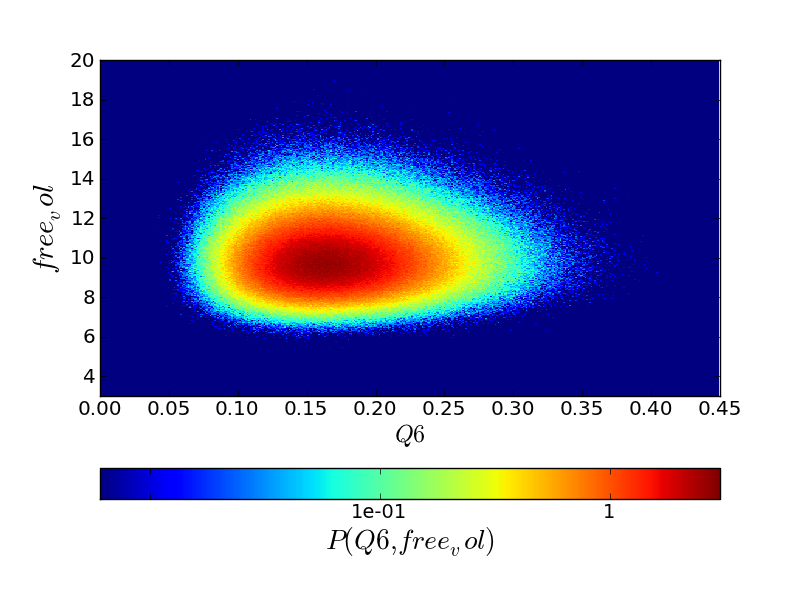
\includegraphics[width=8cm,bb=0 0 576 432]{./figures/mesh_Q6free_vol.png}
 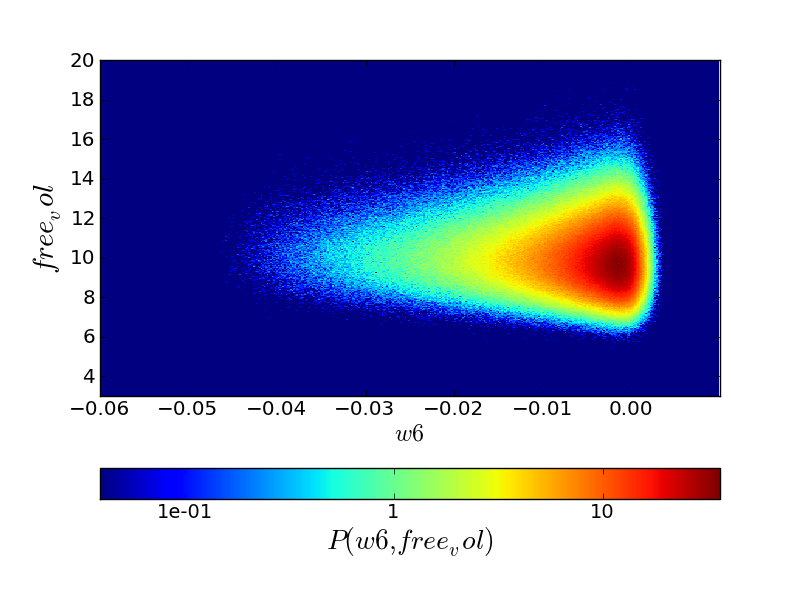
\includegraphics[width=8cm,bb=0 0 576 432]{./figures/mesh_w6free_vol.png}
 % mesh_q6free_vol.png: 800x600 pixel, 100dpi, 20.32x15.24 cm, bb=0 0 576 432
 \caption{Probability distribution functions in the $f_2$,$Q_6$-map (top) and in
the $f_2$,$w_6$-map (bottom) for a metastable fluid with polydispersity $\delta=7\%$
and pressure $\beta p\sigma^3=23$.}
 \label{fig:f2decoupling}
\end{figure}





\subsection{Competition between icosahedral arrangements and crystalline arrangements}

We will now focus on the state point at $\beta p\sigma^3=23$ at different polydispersities to
study the mechanism by which polydispersity disfavours the crystallization transition.

\begin{figure}
 \centering
 \includegraphics[width=8cm]{./figures/Q6_prob.eps}
 \includegraphics[width=8cm]{./figures/w6_prob.eps}
 % Q6_prob.eps: 0x0 pixel, 300dpi, 0.00x0.00 cm, bb=(atend)
 \caption{Probability distribution for order parameters $Q_6$ (top) and $w_6$ (bottom) for
different polydispersities. With increasing polydispersity we note the suppression
of high $Q_6$ regions, i.e. a suppression of bond-orientationally ordered regions. The fraction of
particles in icosahedral environments instead increases with polydispersity, saturating at
high polydispersity.}
 \label{fig:polydispersity}
\end{figure}


In Fig.~\ref{fig:polydispersity} we show the probability distributions for the order
parameters $Q_6$ and $w_6$ and for different polydispersities. It is immediately
evident that, while bond-orientational order is rapidly suppressed with increasing
polydispersity (as shown in the suppressed signal at high $Q_6$), particles in icosahedral
environments are not disfavoured by polydispersity. On the contrary the fraction of
icosahedral particles increases with polydispersity, and saturates at around $\delta=10\%$.

\begin{figure}
 \centering
 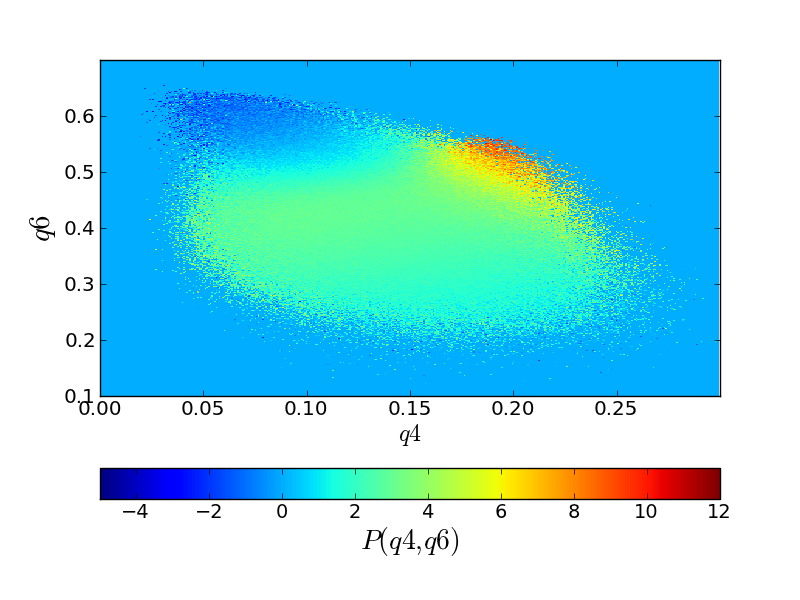
\includegraphics[width=8cm, bb=0 0 576 432]{./figures/mesh_q4q6_007.png}
 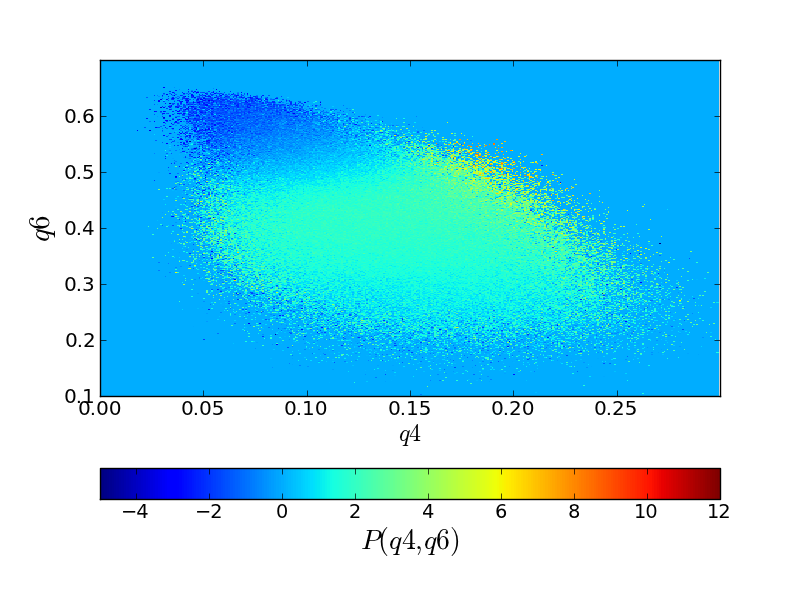
\includegraphics[width=8cm, bb=0 0 576 432]{./figures/mesh_q4q6_015.png}
 % mesh_q4q6_007.png: 800x600 pixel, 100dpi, 20.32x15.24 cm, bb=0 0 576 432
 \caption{Average crystallinity order parameter projected in the $q_4$,$q_6$ space for
the metastable fluid at $\beta p\sigma^3=23$ at $\delta=7\%$ (top) and $\delta=15\%$.}
 \label{fig:q4q6}
\end{figure}


Fig.~\ref{fig:q4q6} shows that the metastable fluid distribution presents both characteristic
structures: icosahedral environments with high $q_6$, low $q_4$ and a low value of the
crystallinity order parameter; bond orientationally ordered regions with high values of
$q_4$, $q_6$ and the crystallinity order parameter. The main difference between the low and
high polydispersity metastable states is the population of the bond-orientationally ordered regions.


In the metastable fluid a competition between bond-ordered regions and icosahedral regions takes
place, with polydispersity favouring the latter. The nature of the competition can be seen
in two-dimensional maps of translational vs orientational order, i.e. $\phi,q_6$ maps.
As was shown in Ref.~\cite{russo_hs}, this plot is very useful in determining the region
of thermodynamic stability of each phase. The calculation is straightforward: for each
configuration, particles are identified as ``fluid'' and ``crystalline'' according to
the criteria described in the methods section. For each subset of particles, the
the average value of the volume fraction
$\phi$ is calculated as a function of the order parameter $q_6$. By looking at the
relative position of the two curves (the one for the fluid particles and the other for the crystalline particles)
the relative stability of the phases can be determined: at each volume fraction,
the stable phase is the one with the higher value of $q_6$. In Fig.~\ref{fig:stability_map}
we compare the curves at $\beta p\sigma^3=17$ and at different polydispersities:
at $0\%$ (monodisperse system, black circles) and at $4\%$ (red squares). The curve for the
crystalline particles is similar at the two considered polydispersities and is reported once
as the dashed line. First we consider he monodisperse case. As shown in the figure,
at low volume fraction, the stable phase is the fluid phase. But at $\phi\cong 55.8\%$ a crossover
occurs and the crystal phase gains stability. This stability is again lost at $\phi\cong 58\%$
because at high $q_6$ values the liquid branch is composed entirely of icosahedral particles.
At polydispersity $\delta=4\%$ the crystalline branch is always metastable to the fluid one.
This is due to an increase in $q_6$ of the fluid branch at high $\phi$, which shifts ``below'' the
crystalline curve. The behaviour of the fluid curve is due to an increased population of
icosahedral particles, which dominate the fluid branch for $q_6\gtrsim 0.5$. The fact that
the crystalline phase loses its metastability window is immediately evident in simulations,
as at this pressure it is not possible to crystallize simulations at $\delta=4\%$, while the
monodisperse simulations have a small nucleation time.

We have thus provided direct evidence that icosahedral particles are responsible for the suppression
of crystallization in polydisperse hard spheres.

\begin{figure}
 \centering
 \includegraphics[width=8cm]{./figures/stability_map.eps}
 % stability_map.eps: 0x0 pixel, 300dpi, 0.00x0.00 cm, bb=(atend)
 \caption{Average $\phi$ as a function of $q_6$ for particles identified as fluid and crystalline.
The circles represent fluid particles in a system at $\beta p\sigma^3=17$ and $\delta=0\%$, while
squares represent fluid particles at the same pressure but at $\delta=4\%$. The dashed curve represents
instead solid particles (this curve is less sensitive to polydispersity and it is reported once).}
 \label{fig:stability_map}
\end{figure}


\bibliographystyle{apsrev4-1}
\bibliography{biblio}

\end{document}
